\documentclass[12pt,titlepage]{article}


\usepackage[utf8]{inputenc} 
\usepackage[a4paper,
            left=2.5cm,
            right=2.5cm,
            top=4cm,
            bottom=2.7cm]{geometry}

\usepackage[english]{babel}
\usepackage[skip=10pt plus2pt, indent=10pt]{parskip}
\begin{document}

\section{Introduction}
Churn prediction is a crucial task in customer relationship management, aiming to identify customers who are likely to discontinue using a service. Accurately predicting churn allows companies to take proactive measures to retain these customers, thereby improving overall business performance.

\section{Data Description}
The dataset used for this task consists of both structured and unstructured data. It contains a total of 10,000 samples, where each sample represents a unique customer. The structured data includes features such as the number of products owned by the customer, their account balance, salary, age, gender, and other information. 

The dataset exhibits a significant class imbalance, which can affect the performance of machine learning models. Out of the 10,000 samples, 8,000 customers did not leave the service, while only 2,000 did. To illustrate the class imbalance, we present a histogram showing the distribution of the two classes

\begin{figure}[h!]
    \centering
    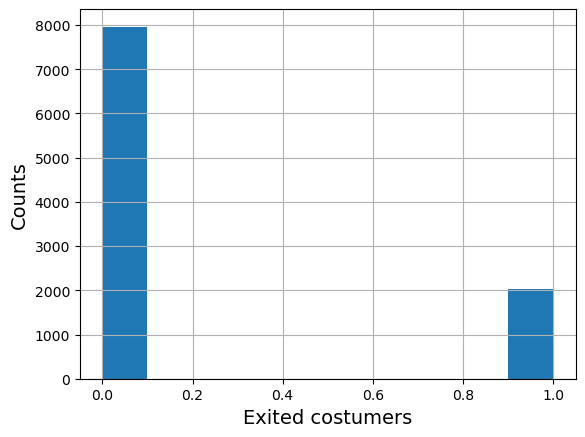
\includegraphics[width=0.7\textwidth]{class_distribution.png}
    \caption{Class Distribution of the Dataset}
    \label{fig:class_distribution}
\end{figure}

To prepare the data for analysis, we first need to encode the categorical features (such as age, gender, country, etc.) into numerical labels. This step is essential because most machine learning algorithms require numerical input. The encoding process transforms each unique category into an integer label. This encoding allows the structured data to be effectively utilized by machine learning models.

\subsection{Encoding Categorical Data}
The following categorical features were encoded into integer labels:
\begin{itemize}
    \item[-] \textbf{Gender:} Encoded as 0 for female and 1 for male.
    \item[-] \textbf{Country:} Each country was assigned a unique integer label.
\end{itemize}
 
Additionally, the dataset contains unstructured data in the form of customer feedback. It is important to note that not all samples have associated customer opinions. For those samples without this entry, we assign a dummy variable of -99.


Customer feedback is a valuable source of unstructured data that can provide insights into customer satisfaction and potential churn risk.
The next steps involve handling the unstructured data and integrating it with the structured data for a comprehensive churn prediction model.
To leverage this data, we perform sentiment analysis to classify the feedback as positive or negative employing the BERT (Bidirectional Encoder Representations from Transformers) model, which is known for its state-of-the-art performance in natural language processing tasks. Specifically, we use the \texttt{BertTokenizer} for tokenizing the feedback text and the \texttt{BertForSequenceClassification} module for classifying each opinion into a 'star rating'. The process involves the following steps:
\begin{itemize}
    \item[-] \textbf{Tokenization:} The \texttt{BertTokenizer} is used to convert the text of each feedback into a format suitable for BERT. This involves breaking the text into tokens and mapping each token to an integer index in the BERT vocabulary.
    \item[-] \textbf{Sequence Classification:} The tokenized text is then passed to the \texttt{BertForSequenceClassification} module. This module is fine-tuned to classify each piece of feedback into one of five categories, corresponding to star ratings ranging from 1 star (the poorest score) to 5 stars (the best score).
\end{itemize}  Once each feedback has been classified into a star rating, we encode these ratings into integer labels. This encoding is similar to the process used for other categorical features:
\begin{itemize}
    \item[-] \textbf{1 star:} Encoded as 0
    \item[-] \textbf{2 stars:} Encoded as 1
    \item[-] \textbf{3 stars:} Encoded as 2
    \item[-] \textbf{4 stars:} Encoded as 3
    \item[-] \textbf{5 stars:} Encoded as 4
\end{itemize}


Once the data is all pre-processed, with a format that algorithms can read, we can look at the correlation between different variables and the probability of customer churn. The following plot shows the correlation between all features in the dataset and their current status (Exited/not Exited). 
%\begin{figure}[h!]
%    \centering
%    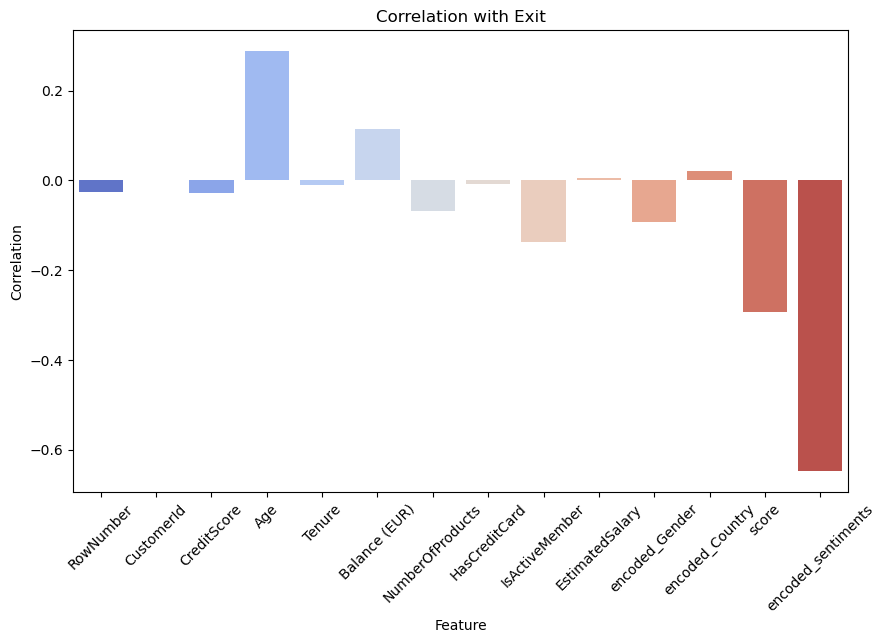
\includegraphics[width=0.9\textwidth]{Figures/correlation_matrix.png}
%    \caption{Correlation Matrix of Features and Exit Probability}
%    \label{fig:correlation_matrix}
%\end{figure}

Customer feedback is an important feature in predicting churn. It provides valuable insights into customer satisfaction, which can be indicative of their likelihood to leave the service. However, our analysis revealed some interesting findings. We found instances where customers gave excellent ratings (5 stars) but still left the service. Manual verification confirmed the high ratings, suggesting that despite positive feedback, these customers decided to churn. Conversely, some customers gave poor ratings (1 or 2 stars) but did not leave the service. This indicates that negative feedback does not always lead to churn.

These findings highlight the complexity of human behavior. While customer feedback is a relevant feature, it is not an infallible predictor of churn. Other factors, potentially unaccounted for in the dataset, may influence a customer's decision to leave or stay. 

\section{Main Results}
To address the churn prediction task, we employed two machine learning approaches: Gradient Boosting and a Neural Network. Other algorithms were also tested, but Gradient Boosting provided the best results. Both algorithms were optimized using Optuna, a hyperparameter optimization framework. Optuna allows for efficient exploration of the hyperparameter space to find the best performing settings for each model.

The performance of the models was evaluated using two primary metrics:
\begin{itemize}
    \item \textbf{ROC Curve:} The Receiver Operating Characteristic (ROC) curve is a graphical representation of the true positive rate (sensitivity) versus the false positive rate (1-specificity) at various threshold settings. The area under the ROC curve (AUC) provides a single metric to evaluate the overall performance of the model, with higher values indicating better performance.
    \item \textbf{Confusion Matrix:} The confusion matrix provides a detailed breakdown of the model's predictions, showing the number of true positives, true negatives, false positives, and false negatives. This helps in understanding the model's performance on each class.
\end{itemize}

\subsection{Gradient Boosting Results}
The Gradient Boosting model achieved an AUC of 0.91. The confusion matrix indicated the following performance:
\begin{itemize}
    \item \textbf{True Negatives:} 95\% of the customers who did not leave the service were correctly predicted.
    \item \textbf{True Positives:} 70\% of the customers who left the service were correctly predicted.
\end{itemize}

\begin{figure}[h!]
    \centering
    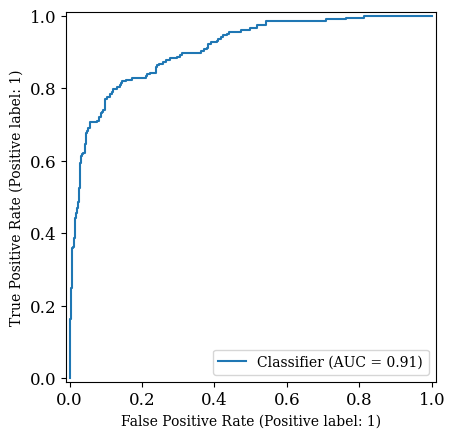
\includegraphics[width=0.5\textwidth]{Figures/roc_curve_gb.png}
    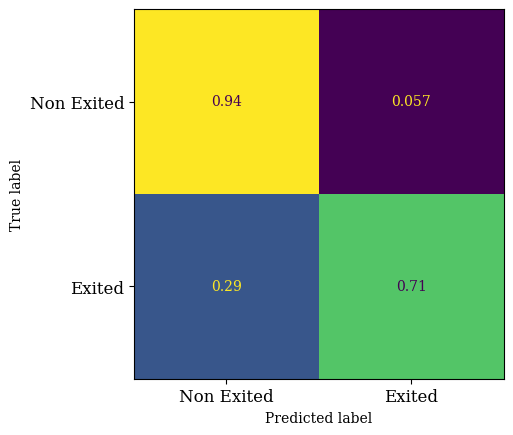
\includegraphics[width=0.7\textwidth]{Figures/confusion_matrix_gb.png}
    \caption{ROC Curve for Gradient Boosting}
    \label{fig:roc_curve_gb}
\end{figure}


\subsection{Neural Network Results}
The Neural Network model yielded similar results, though slightly worse:
\begin{itemize}
    \item \textbf{AUC:} Approximately 0.90.
    \item \textbf{True Negatives:} 90\% of the customers who did not leave the service were correctly predicted.
    \item \textbf{True Positives:} 65\% of the customers who left the service were correctly predicted.
\end{itemize}

\begin{figure}[h!]
    \centering
    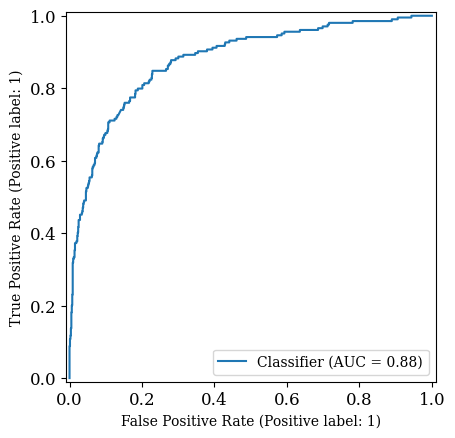
\includegraphics[width=0.7\textwidth]{roc_curve_nn.png}
    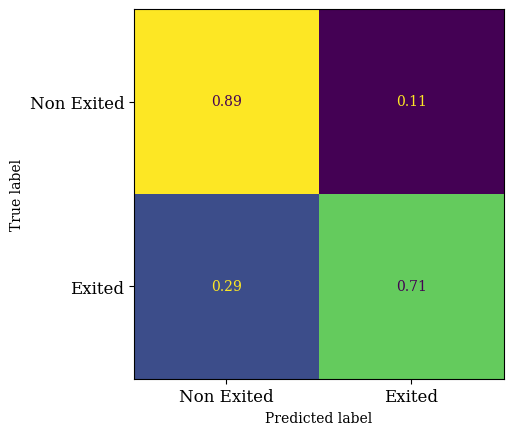
\includegraphics[width=0.7\textwidth]{confusion_matrix_nn.png}
    \caption{ROC Curve for Neural Network}
    \label{fig:roc_curve_nn}
\end{figure}

The slightly lower performance of the Neural Network could be attributed to its sensitivity to dummy variables and the need for data normalization. Although normalization was performed, further optimization might improve results.

\subsection{Discussion on Prediction Imperfection}
Despite the overall strong performance of the models, the churn prediction is not perfect. One contributing factor is the inherent unpredictability of human behavior. As previously discussed, even customers with excellent feedback ratings might leave the service, and those with poor ratings might stay. This unpredictability adds a layer of complexity that machine learning models may not fully capture.

\end{document}




\end{document}